\documentclass[11pt]{texMemo-gibbons}
\usepackage[english]{babel}
\usepackage{graphicx}
\usepackage{blindtext}
\usepackage{amsmath,amssymb,units}
\usepackage{siunitx}
\usepackage[outdir=./]{epstopdf}
\usepackage{subfigure}
\memostudent{Ty Davis}
\memocourse{ECE 3210}
\memosubject{Lab 9, Filter Design}
\memodate{\today}
\logo{
\includegraphics[width=0.5\textwidth]{ece_horiz.pdf}}

\begin{document}
\maketitle

\section{Introduction}
\label{sec:introduction}

In this lab we are tasked with designing a low-pass
filter that satisfies a set of requirements. Our target
satisfies the following specifications:


\begin{itemize}
 \item Pass band is 0 Hz to 7.5 kHz
 \item Stop band is 10 kHz to $\infty$
 \item Max ripple in the pass band is 1.5 dB
 \item Minimum attenuation in the stop band is -24 dB
\end{itemize}


\section{Theory}
\label{sec:theory}

We decided to build a Chebyshev filter, and after using 
the scipy function cheb1ord, we found
the transfer function of the filter, shown in Eq.~\ref{eq:transfer}.

\begin{equation}
  H(s) = \frac{2.2613 \times 10 ^ {22}}{s^5 + 3.7766 \times 10 ^ 4 s ^ 4 + 3.4889 \times 10 ^ 9 s ^ 3 + 8.4179 \times 10 ^ {13} s ^ 2 + 2.4863 \times 10 ^ {18} s + 2.2613 \times 10 ^ {22}}
  \label{eq:transfer}
\end{equation}

The results of the transfer function are shown in Fig.~\ref{fig:calc}.

The denominator of this function is a fifth order expression, so we used
a fifth order Chebyshev filter, which is shown in Fig.~\ref{fig:circuit}

This is essentially just two Sallen-key filter circuits just like
the one from lab 8 stacked with a first order filter.

When selecting the component values for the circuit we used
the equations from the last lab, but for different values of
$\omega_c$ depending on the stage of the Chebyshev filter. The 
variables in those equations can be expressed in terms of
the resistors and capacitors with the following equations:

\[
  \omega_c^2 = \frac{1}{R_1 \cdot R_2 \cdot C_1 \cdot C_2}
\]

\[
  \omega_c \zeta = \frac{2 R_1}{R_1 \cdot R_2 \cdot C_1}
\]

We chose to select common resistor values for $R_1$ and $R_2$,
and make them equal to each other, because the problem wasn't 
fully defined and left some room for our choice. Then we 
had sympy solve for given resistances until we found a set 
of capacitances that would work for each stage of the filter.

Table~\ref{tab:components} shows the values that we decided to use
to build the filter.



\section{Results}
\label{sec:results}

The results of the Multisim simulation are shown in Fig.~\ref{fig:sim}.
Note that the results match the specifications of the circuit. As do 
the results from the prototyped circuit shown in Fig.~\ref{fig:meas}.

We did not include a graph of the poles or zeros because there 
were none from this filter.


\section{Discussion and Conclusions}
\label{sec:conclusions}

Our design of a filter was successful. We built a filter that had 
a pass band of 0 to 7.5~kHz and the stop band was from 10~kHz to $\infty$.
It is difficult to see in the graph, but the ripple was under 2~dB, only just a 
built over 1.5~dB.

\clearpage

\begin{figure}[h!]
  \centering
  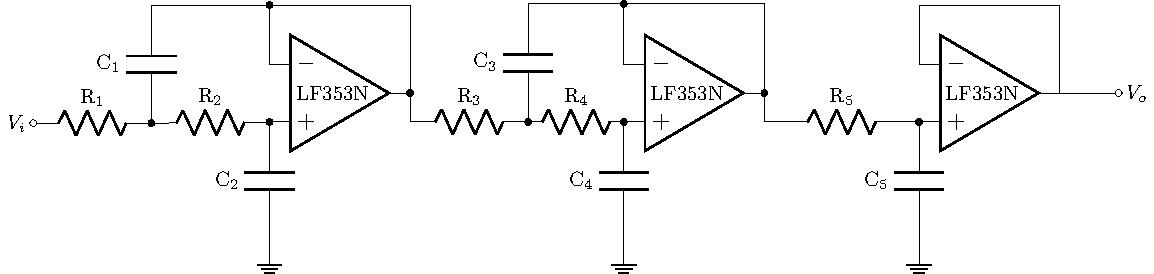
\includegraphics[width=\textwidth]{../circuits/circuit_blank.pdf}
  \caption{Fifth Order Chebyshev Filter}
  \label{fig:circuit}
\end{figure}

\begin{table}[h!]
  \begin{tabular}{c c}
    \textbf{Component} & \textbf{Value} \\
    \bottomrule
    $R_1$ & 4.7~\si{\kohm} \\
    $R_2$ & 4.7~\si{\kohm} \\
    $C_1$ & 59~\si{\nF} \\
    $C_2$ & 357~\si{\pF} \\
    $R_3$ & 100~\si{\kohm} \\
    $R_4$ & 100~\si{\kohm} \\
    $C_3$ & 1~\si{\nF} \\
    $C_4$ & 104~\si{\pF} \\
    $R_5$ & 330~\si{\kohm} \\
    $C_6$ & 259~\si{\pF} \\
  \end{tabular}
  \centering
  \caption{Component Values}
  \label{tab:components}
\end{table}


\begin{figure}[h!]
  \centering
  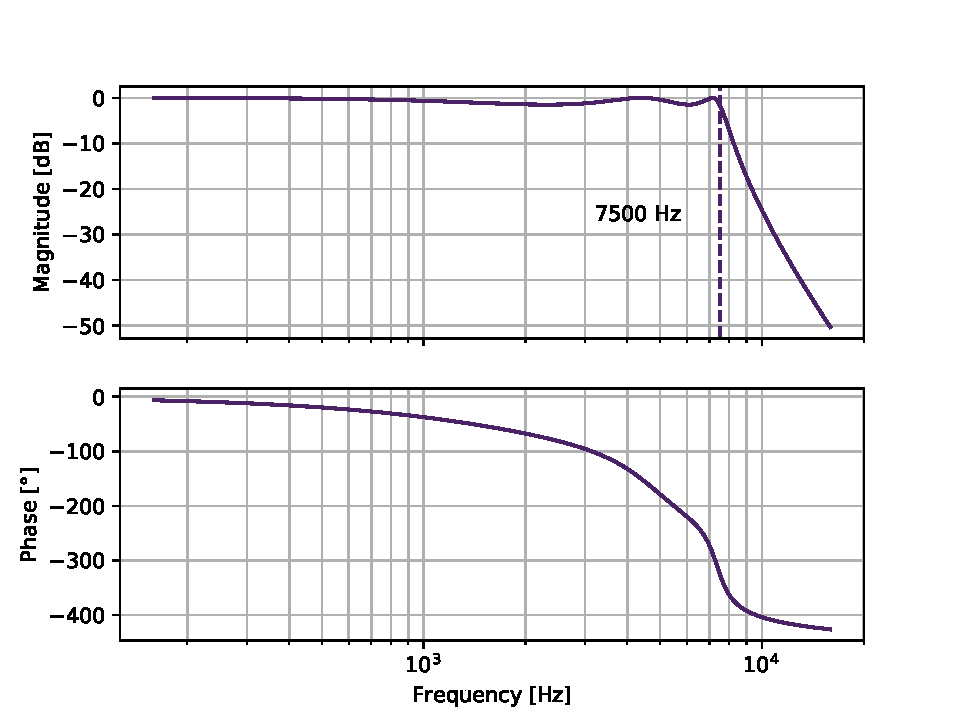
\includegraphics[width=0.7\textwidth]{../plots/calculation_results.pdf}
  \caption{Python Calculation Results}
  \label{fig:calc}
\end{figure}


\begin{figure}[h!]
  \centering
  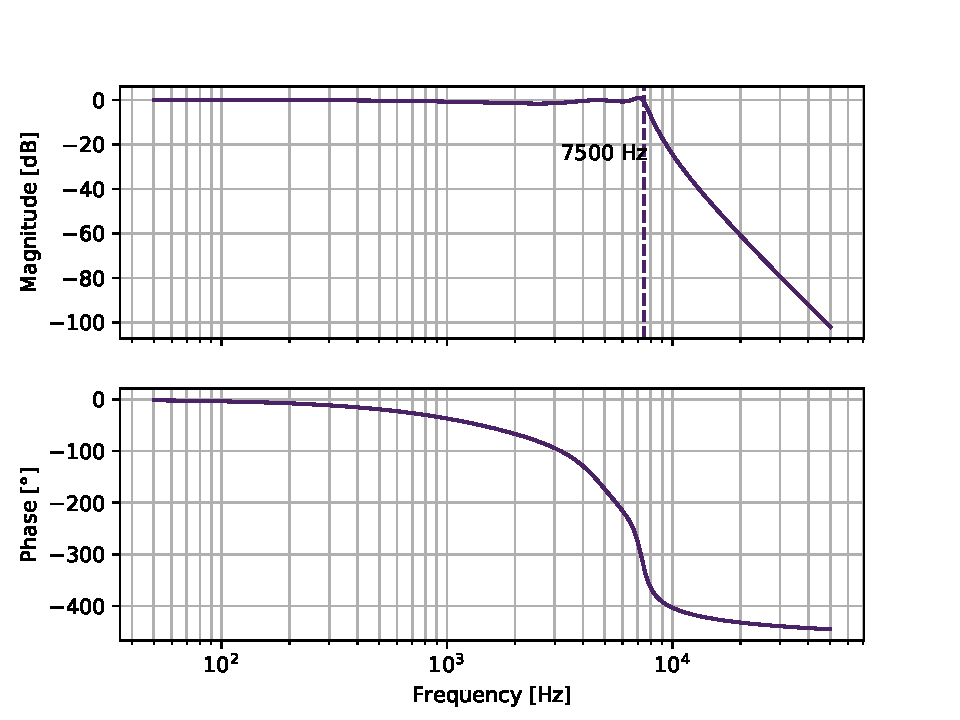
\includegraphics[width=0.7\textwidth]{../plots/simulation_results.pdf}
  \caption{Multisim Simulation Results}
  \label{fig:sim}
\end{figure}

\begin{figure}[h!]
  \centering
  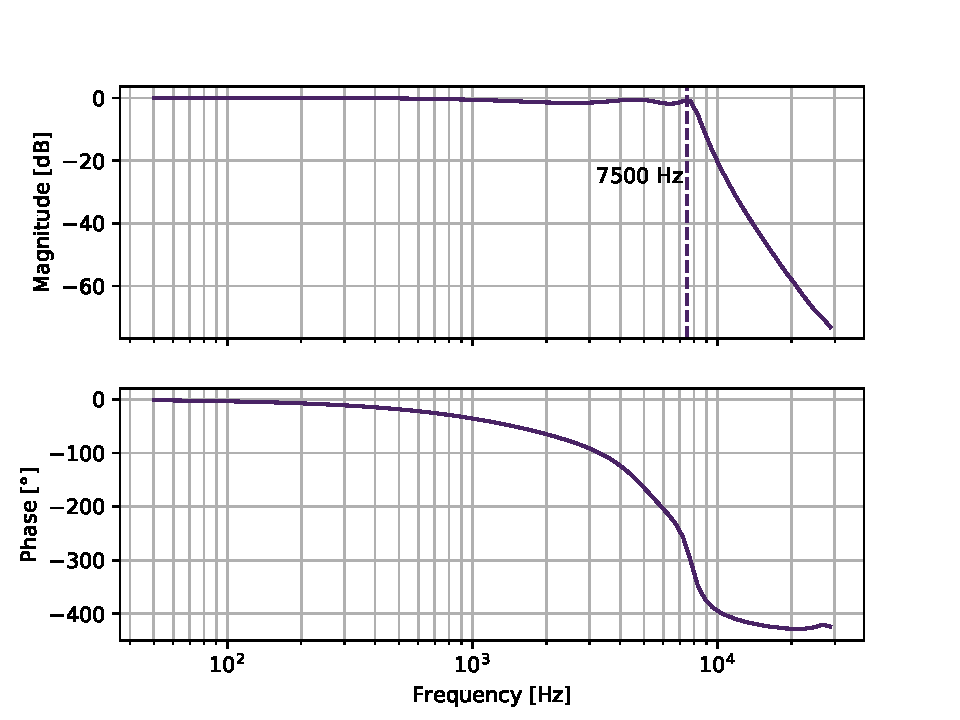
\includegraphics[width=0.7\textwidth]{../plots/measurement_results.pdf}
  \caption{Prototyped Measurement Results}
  \label{fig:meas}
\end{figure}

\end{document}
